\documentclass{article}
\usepackage{polski}
\usepackage[utf8]{inputenc}

%s\usepackage[margin=2.5cm]{geomtry}

\usepackage{graphicx}    % Pakiet pozwalający ,,wklejać'' grafikę...

\usepackage{amsmath,amssymb,amsfonts,amsthm,mathtools}
                               % Dołączamy zestaw różnych przydatnych znaczków ...
\DeclareMathOperator{\arccosh}{arccosh}
% dane autora
\author{Wiktor Pilarczyk}
\title{Pracownia z analizy numerycznej\\\small{Zadanie: P1.25}\\\large{Prowadzący: Witold Karczewski}}
\date{\today}
% początek dokumentu
\begin{document}
\maketitle
\section{Wielomiany i Algorytm Clenshawa}
\indent Szereg Taylora umożliwia dowoloną funkcję f $\in \mathrm{C}^{n+1}$ przybliżyć za pomoca wielomianu stopnia n. Wielomiany ze względu na swoje własności takie jak różniczkowalność lub ciąglość, znalazły szerokie zastosowanie  m.in. w analizie matematycznej lub ekonomii. Ważnym aspektem jest liczenie pochodnej wielomianu, która pozwala na dokladniejszą analizę zachowania się funkcji.\\
\indent Wielomiany Czebyszewa jest to zbiór wielomianów zadanych rekurencją:
{\begin{center}
$T_0(x) = 1$\hspace{0,6cm
$T _1(x) = x$\\
\end{center}}
\begin{equation}
T_{k}(x)=2x\ T_{{k-1}}(x)-T_{{k-2}}(x)
\end{equation}
Albo wzorem trgonometrycznym:

\begin{equation} 
    T_{k}(x)=\left\{
                \begin{array}{ll}
                  \cos(k \arccos x) \ dla \  |x| \leqslant 1\\
                  \cosh(k \arccosh x) \ dla \  x > 1\\
                  \cosh(k \arccosh -x) \ dla \  x < -1\\
                \end{array}
              \right.
\end{equation}
Wielomiany te są wzajemnie ortogonalne, przez co tworzą bazę przestrzeni wielomianów.\\
\indent Algorytm Clenshawa został skonstruowany do rekurencyjnego obliczania liniowej kombinacji wielomianów Czebyszewa, ale ogólnie stosuje się go do funkcji definiowalnych za pomocą trójtermowego równania rekurencyjnego:
$$s_n := \sum_{i=1}^{n} w_i\ P_i$$\\ 
gdzie $w_i$ są wspołczynnikami, a $P_k$ ciągiem wielomianów zadany wzorem rekurencyjnym:
{\begin{center}
$P_0(x) = a_0$\hspace{0.6cm}
$P_1(x) = (a_1x-b_1)P_0(x)$\\
\end{center}}
\begin{equation}
    P_{k}(x)=(a_kx-b_k)P_{k-1}(x)-c_kP_{k-2}(x) \hspace{0,8cm} (k = 2,3,...)\\
\end{equation}
przy czym $a_k, b_k, c_k$ są danymi stałymi. 
\newpage
Algorytm Clenshawa można też wyliczyć za pomocą zadanej rekurencji:\\
{\begin{center}
    $B_{n+1}(x) = 0$\hspace{0.6cm}
    $B_{n+2}(x) = 0$\\
\end{center}}
\begin{equation}
    B_{k}(x)=w_k+(a_{k+1}x-b_{k+1})B_{k+1}(x)-c_{k+2}B_{k+2}(x) \hspace{0,8cm} (k = n,n-1,...,0)\\
\end{equation}
\begin{equation*}
    s_n(x)=a_0B_0
\end{equation*}
\subsection{Dowód równoważności algorytmów (3) i (4)}
Teza: $$\sum_{i=1}^{n} w_iP_i = a_0B_0$$
Lemat: 
\begin{equation}
    P_kB_k-c_{k+1}B_{k+1}P_{k-1}=\sum_{i=k}^{n} w_iP_i
\end{equation}
Przeprowadzony zostanie dowód indukcyjny lematu po k.\\
Baza: $k = n$
$$P_nB_n-c_{n+1}B_{n+1}P_{n-1}=P_nB_n=P_nw_n=\sum_{i=n}^{n} w_iP_i$$
Założenie Indukcyjne: 
\begin{equation}
    P_kB_k-c_{k+1}B_{k+1}P_{k-1}=\sum_{i=k}^{n} w_iP_i
\end{equation}
Teza Indukcyjna:
\begin{equation}
    P_{k-1}B_{k-1}-c_kB_kP_{k-2}=\sum_{i=k-1}^{n} w_iP_i
\end{equation}
\begin{proof}
    $$P_{k-1}B_{k-1}-c_kB_kP_{k-2}=^{z\ def\ B}$$
    $$=P_{k-1}(w_{k-1}+(a_kx-b_k)B_k-c_{k+1}B_{k+1})-c_kB_kP_{k-2}=$$
    $$=P_{k-1}w_{k-1}+B_k((a_kx-b_k)P_{k-1}-c_kP_{k-2})-c_{k+1}B_{k+1}P_{k-1}=$$
    $$=P_{k-1}w_{k-1}+B_kP_{k}-c_{k+1}B_{k+1}P_{k-1}=P_{k-1}w_{k-1}+\sum_{i=k}^{n} w_iP_i=^{(6)}$$
    $$=\sum_{i=k-1}^{n} w_iP_i$$
    \newpage
    Na mocy zasady o indukcji $$P_kB_k-c_{k+1}B_{k+1}P_{k-1}=\sum_{i=k}^{n} w_iP_i$$
    Rozpisując $a_0B_0$ oraz korzystając z lematu (5) otrzymujemy:
    $$a_0B_0=a_0w_0+a_0(a_1x-b_1)B_1-a_0c_2B_2=w_0P_0+P_1B_1-c_2B_2P_0=$$
    $$=w_0P_0+\sum_{i=1}^{n} w_iP_i=\sum_{i=0}^{n} w_iP_i$$
\end{proof}
\section{Obliczenia}
\subsection{Wielomiany Czebyszewa}
Porównujemy dwa algorytmy (3) i (4) za pomocą, których zostanie obliczona pochodna wielomianu Czebyszewa. Na podstawie wzoru trygonometrycznego (2) obliczamy pochodną wielomianu:
\begin{equation} 
    T'_{k}(x)=\left\{
                \begin{array}{ll}
                  \frac{-k \sin(k \arccos x)}{\sqrt{1-x^2}} \ dla \  |x| \leqslant 1\\
                  \frac{k \sinh(k \arccosh x)}{\sqrt{x^2-1}} \ dla \  x > 1\\
                  \frac{(-1)^{k+1}k \sinh(k \arccosh (-x))}{\sqrt{x^2-1}} \ dla \  x < -1\\
                \end{array}
              \right.
\end{equation}
za pomocą tego wzoru będzie wyliczana wartość, którą powinny otrzymać algorytmy.\\
Dla współczynników $a_0=a_1=1$, $c_0=c_1=0$, $b_k=0$, $c_l=1$ i $a_l=2$ gdzie $k\in \mathrm{N}$ i $n>1$ algorytmy (3) i (4) obliczają $P_k$ które są kolejnymi wielomianami Czebyszewa (z (1)).\\ Jeżeli chcemy obliczyć $P'_k$. Dla algorytmu (3) otrzymujemy:
\begin{equation} 
    P'_{k}(x) = a_{k}P_{k-1}(x) + (a_{k}x - b_{k})P'_{k-1}(x) - c_{k}P'_{k-2}(x)
\end{equation}
a dla (4):
\begin{equation} 
    B'_{k}(x) = a_{k+1}B_{k+1}(x) + (a_{k+1}x - b_{k+1})B'_{k+1}(x) - c_{k+2}B'_{k+2}(x)
\end{equation}
Dla obu algorytmów będziemy obliczać wartość dwóch poprzednich wyrazów, aby uzyskać następny. Należy zwrócić uwagę, że istnieje też inna metoda polegająca na wyliczeniu wspołczynników przy odpowiednich potęgach wielomianu, a następnie obliczeniu pochodnych wielomianu dla kolejnych wyrazów wielomianu.
\begin{table}
    \centering
    \begin{tabular}{ |p{2cm}|p{1.8cm}|p{1.1cm}|p{4.5cm}|p{4.5cm}|}
     \hline
     Indeks\ \ \ \ Wielomianu & Przedział & Iteracja & Średni Błąd Względny dla Clen1 & Średni Błąd Względny dla Clen2\\
     \hline
     2 & 2 - 100000 & 100 & 4.30668983454543547602e-19 & 4.30668983454543547602e-19\\
    \hline
     2 & -0.99 - 0.99 & 0.001 &  0.40550677751445726477 & 0.40550677751445726477\\
     \hline
     2 & -2 - -100000 & -100 & 4.30668983454543547602e-19 & 4.30668983454543547602e-19\\
     \hline
     20 & 2 - 100000 & 100 & 5.40279468529885346981e-18 & 5.40608687015868195457e-18\\
    \hline
     20 & -0.99 - 0.99 & 0.001 &  0.405506777514457257642 & 0.405506777514457257588\\
     \hline
     20 & -2 - -100000 & -100 & 5.40279468529885346981e-18 & 5.40608687015868195457e-18\\
     \hline
     39 & 2 - 100000 & 100 & 1.03496271173449142695e-17 & 1.03573948612679605078e-17\\
    \hline
     39 & -0.99 - 0.99 & 0.001 &  0.40558815601965413555 & 0.405588156019654135631\\
     \hline
     39 & -2 - -100000 & -100 & 1.03496271173449142695e-17 & 1.03573948612679605078e-17\\
     \hline
    \end{tabular}
    \caption{Pochodna Wielomianu Czebyszewa dla precyzji 64 bitowej}
\end{table}
\subsection{Dowolny wielomian}
\indent Ponieważ wielomiany Czebyszewa tworzą bazę wielomianów, można dowolny wielomian przedstawić za pomocą kombinacji liniowej tychże wielomianów. Niech:
\begin{equation}
    W(x) = x^5 + 4x^4 + - x^3 - 3/2
\end{equation}
wtedy
$$W(x) = \frac{T_5}{16} + \frac{T_4}{2} + \frac{T_3}{16} + T_2 - \frac{T_1}{8}$$
Pochodna tego wielomianu wynosi:
\begin{equation}
    W'(x) = 5x^4 + 16x^3 + - 3x^2
\end{equation}
Otrzymane wyniki:\\
%\begin{table}
    %\centering
    \begin{tabular}{ |p{3cm}|p{1.1cm}|p{4.5cm}|p{4.5cm}|}
     \hline
     Przedział & Iteracja & Średni Błąd Względny dla Clen1 & Średni Błąd Względny dla Clen2\\
     \hline
     -100050 - 100050 & 100 & 6.75328483818304807646e-09 & 6.75328483818300485506e-09\\
     \hline
     -1 - 1 & 0.001 & 142.584756274333033954 & 142.584756274333033954\\
     \hline
    \end{tabular}
 %   \caption{Pochodna Wielomianu dla precyzji 64 bitowej}
%\end{table}

\section{Uwarunkowanie zadania}

Uwarunkowanie zadania zależy od funkcji, którą mamy obliczyć, a nie od sposobu w jaki jest obliczana.
Wskaźnik uwarunkowania zadania jest wielkością charakteryzującą wpływ zaburzeń danych na odkształcenie rozwiązania:
\begin{equation}
    C_{f}(x) =  \frac{f(x)}{f'(x)}
\end{equation}
 Należy zwrócić uwagę na ten aspekt, aby wyniki były rzetelne.

\subsection{Pochodne wielomianów Czebyszewa}
Aby sprawdzić dla jakich x zadanie jest źle uwarunkowane należy sprawdzić kiedy:
\begin{equation} 
    \lim_{x\to x_0} \frac{T'_{k}(x)}{T''_{k}(x)}=\infty
\end{equation}
lub
\begin{equation} 
    \lim_{x\to x_0} \frac{T'_{k}(x)}{T''_{k}(x)}=-\infty
\end{equation}
Zadanie jest dobrze uwarunkowane.
\subsection{Dowolny wielomian}
Obliczając pochodną funkcji (12) otrzymujemy:
\begin{equation}
    W'(x) = 20x^3 + 48x^2 -6x
\end{equation}
Obliczając wskaźnik uwarunkowania zadania (13) otrzymujemy:
\begin{equation}
    C_{f}(x) =  \frac{x(x + \frac{8}{5} + \frac{\sqrt{79}}{5})(x + \frac{8}{5} - \frac{\sqrt{79}}{5}}{(x + \frac{6}{5} + \frac{\sqrt{\frac{87}{2}}}{5})(x + \frac{6}{5} - \frac{\sqrt{\frac{87}{2}}}{5})}
\end{equation}
więc dla x w pobliżu $-\frac{6}{5} - \frac{\sqrt{\frac{87}{2}}}{5}$ oraz $-\frac{6}{5} + \frac{\sqrt{\frac{87}{2}}}{5}$.
\section{Analiza wyników}
\subsection{Wielomiany Czebyszewa}
\indent Porównując otrzymane wyniki, można wywnioskować, że dla płytkiej rekurencji jaką jest otrzymanie 2-giego wielomainu Czebyszewa błędy względne algorytmów są identyczne, lecz już dla większych indeksów (głebyszch wywołań) funkcja Clen1 (algorytm (3)) otrzymuje nieco lepsze wyniki niż Clen2 (algorytm (4)).\\
\indent Warto zwrócić uwagę na duży błąd względny w przedziale -0.99 - 0.99, który jest spowodowany dużymi zmianami pochodnej wielomianu dla małych zaburzeń, miejsca zerowe w wielomianie znajdują się w przedziale od $(-1,1)$. Zauważalne jest to na krańcach przedziału, dla których błąd względny jest wielkości $~$ 0.8. Wynika to z faktu, że dla pochodnej wielomianu Czebyszewa (indeksu $k > 2$):
$$\lim_{x \to 1} T'_k(x) = \infty$$
$$\lim_{x \to -1} T'_k(x) = -\infty$$
\begin{figure}[h]
\centering
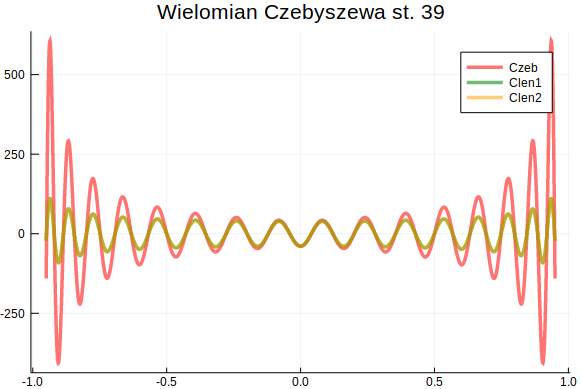
\includegraphics[width=12cm,height=7cm]{wykresczeb.png}
\end{figure}
\subsection{Dowolny wielomian}
\indent Oba algorytmy z dużą dokładnością obliczają pochodną wielomianu. Średni błąd względny dla przedziału $[-1, 1]$ jest wysoki, ponieważ w tym przedziale znajdują się punkty, w których zadanie jest źle uwarunkowane, jednym z nich jest $-\frac{6}{5} + \frac{\sqrt{\frac{87}{2}}}{5}$ w przybliżeniu wynosi $-0.119$ dla punktu $-0.1$ średni błąd względny wynosi $\approx 918$, a także w miejscach gdzie funkcja przyjmuje wartości bliskie 0 - $x = 0.18$ błąd względny wynosi $\approx 345$.
\begin{figure}[h]
\centering
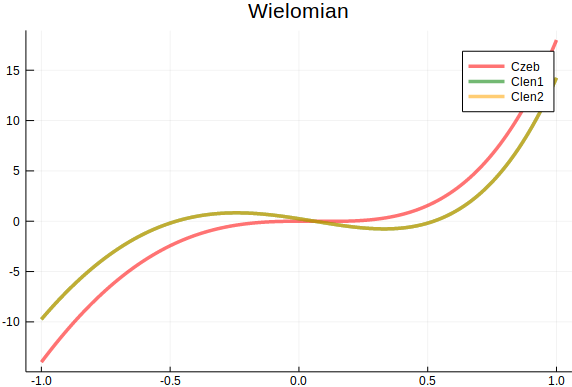
\includegraphics[width=12cm,height=7cm]{wykreswiel.png}
\end{figure}
\begin{thebibliography}{99}
\bibitem{} D. Kincaid, W. Cheney:
\emph{Analiza numeryczna, WNT, 2005},
\bibitem{} G. Dahlquist, A. Bjorck:
\emph{Numerical Methods in Scientific Computing, Vol.I, SIAM, 2008.},
\bibitem{} M. Dryja, J. i M. Jankowscy:
\emph{Przegląd metod i algorytmów numerycznych cz. 2, WNT, 1988},

\end{thebibliography}
\end{document}
